\documentclass[12pt]{article}%

%============================================================================
% Assignment Information

\def\assignmentName { Project 3 - Website Analysis                      }
\def\className      { CSE 321: Internet and Web Programming             }
\def\studentName    { Noah Schoonover \\ Myles Willis \\ Adam Schmidt   }
\def\studentEmail   {  }
\def\dueDate        { September 16, 2021                                }
\def\semesterDate   { Fall 2021                                         }

%============================================================================
% Packages

\usepackage{tabularx, makecell}
\usepackage{setspace}
\usepackage[shortlabels]{enumitem}
\renewcommand{\thesubsection}{\thesection.\alph{subsection}}
\usepackage[a4paper, top=2.5cm, bottom=2.5cm, left=1.5cm, right=1.5cm]{geometry}
\usepackage{amsmath, amssymb}
\usepackage{float, graphicx}
\usepackage[bottom]{footmisc}

%============================================================================
% User Defined Commands

\newcommand{\itemAt}[1]{\setcounter{enumi}{#1 - 1}\item}
\newcommand{\ntab}{\hspace*{1cm}}

%============================================================================
% Headers and Document Setup

\doublespacing

%============================================================================
\begin{document}
%============================================================================

%---------------------------------------------------------------------
% Title

\begin{singlespace}
\title{ \assignmentName }
\author{ \studentName \\ {\small \studentEmail} \\ {\it \className}}
\date{\dueDate (\semesterDate)}
\maketitle
\end{singlespace}

%---------------------------------------------------------------------
% Document


\begin{itemize}
    \item Theme:

    The goal of this project is to simplify the way contact information and social accounts are shared with the people you meet.
    we aim to provide users with the ability to share their "Zolink", a personalized contact card web page that can be used for personal,
    business and networking purposes, without the need for their own server or domain. We hope to allow users to share complete
    contact cards with one link, QR code, or Zolink username.

    \item Group Name: Zolink
    \item Group Members:
    \begin{itemize}
    	\item Noah Schoonover
    	\item Myles Willis
    	\item Adam Schmidt
    \end{itemize}
\end{itemize}


\section{Background}

Nearly everyone has accounts on social media platforms such as Instagram, LinkedIn, Snapchat, etc. When you meet someone it can
be a pain to share each of these accounts individually in addition to other contact information. Why not have a way to share the
information you want all at once?


\section{Website Analysis}
    \begin{enumerate}[2.a.]

        \item Five existing websites found which offer services for creating digital contact/ business cards include: CardURL, OVOU Card, Switchit, vCard Maker and HiHello. Each of these sites vary in their execution of this service in their use of the unique features they offer to customers and the way they envision their system being used. The features of each of these sites is listed below.

        \begin{enumerate}
            \item [--] \textbf{CardURL (Paid service subscription)}

            \begin{itemize}
                \item View and download count tracking (card statistics)
                \item Notify contacts of modifications
                \item Create multiple cards with varying information
                \item Direct import to contact lists on mobile devices
                \item Short, personalized URL and QR code
                \item Profile photo
            \end{itemize}

            \item [--] \textbf{OVOU Card (Paid physical card)}


            \begin{itemize}
                \item Physical card with NFC and QR code
                \item Customize-able card and personal page
                \item Add directly to contacts on mobile devices
                \item Host individual URL as public web-page
                \item Choose username or have one generated through OVOU site
                \item Profiles do not show on search engines
            \end{itemize}

            \item [--] \textbf{Switchit (Paid service subscription + App)}

            \begin{itemize}
                \item Add media (Video and Images)
                \item Smart Contact Manager
                \item Fully developed app to create and share profiles
                \item Personalized notes on contacts users receive
                \item Business card scanner (Photo to digital)
                \item Sync with Outlook, Google Calendar, iCloud Calendar
                \item File attachment (PDF fill forms , documents ,etc)
                \item Call and text contacts using the app
            \end{itemize}

            \item [--] \textbf{vCard Maker (Free)}
            \begin{itemize}
                \item Add job/social network information
                \item Lacks QR code
                \item Lacks Unique link/online hosting
                \item (.vcf) file creation and download
                \item Attach .vcf file to emails and messages to be downloaded
            \end{itemize}

            \item [--] \textbf{HiHello (Paid service subscription + App)}

            \begin{itemize}
                \item Mobile app
                \item QR code, NFC tag sharing
                \item Address book
                \item Import google contacts
                \item Paper business card transcriptions
                \item Custom colors/page customization
                \item Personalized link
                \item Include files and profile videos
                \item Sync with Outlook and Google services
            \end{itemize}
        \end{enumerate}

        \item We are aiming to:
        \begin{itemize}
        	\item Allow users to create an account and add the information they desire on their Zolink.
        	\item Allow users to create multiple contact cards with different purposes.
        	\item Have an option to make contact cards public or private.
        	\item Create a unique URL and QR code for every card so that the user will be able to share these cards easily.
        \end{itemize}
        \item
    \end{enumerate}

\begin{center}
    \begin{tabular}{|l|l|l|l|l|l|l|}
        \hline
         & Zolink & CardURL & OVOU Card & Switchit & vCard Maker & HiHello \\
         \hline
        QR Code & V & V & V & X & X & V \\
        \hline
        Unique URL & V & V & V & X & X & V \\
        \hline
        Multiple Cards & V & V & X & X & X & X \\
        \hline
        Add personal info & V & X & V & V & V & V \\
        \hline
        Page Customization & V & O & V & O & X & V \\
        \hline
        Import to mobile & X & V & V & V & X & V \\
        \hline
        Physical card & X & X & V & X & X & X \\
        \hline
        File Upload & V & X & X & V & V & V \\
        \hline
        Public/Private cards & V & V & X & V & X & X \\
        \hline
    \end{tabular}
\end{center}

\clearpage
\section{Storyboard} 

\begin{enumerate}[a.]
    \item The user-base for Zolink will include nearly any demographic, as almost anyone can make use of a digital business card. Most people have multiple social media accounts as well as email addresses, phone numbers, and a physical address. Simply put, anyone who has the ability to use the web and create an account will find Zolink useful. 
    
    All users will have the same role and capabilities on Zolink, aside from the developers who will be able to moderate user information if needed.
    
    \item
\end{enumerate}

\begin{center}
    {\bf \Large Welcome Page}
    \makebox[\textwidth]{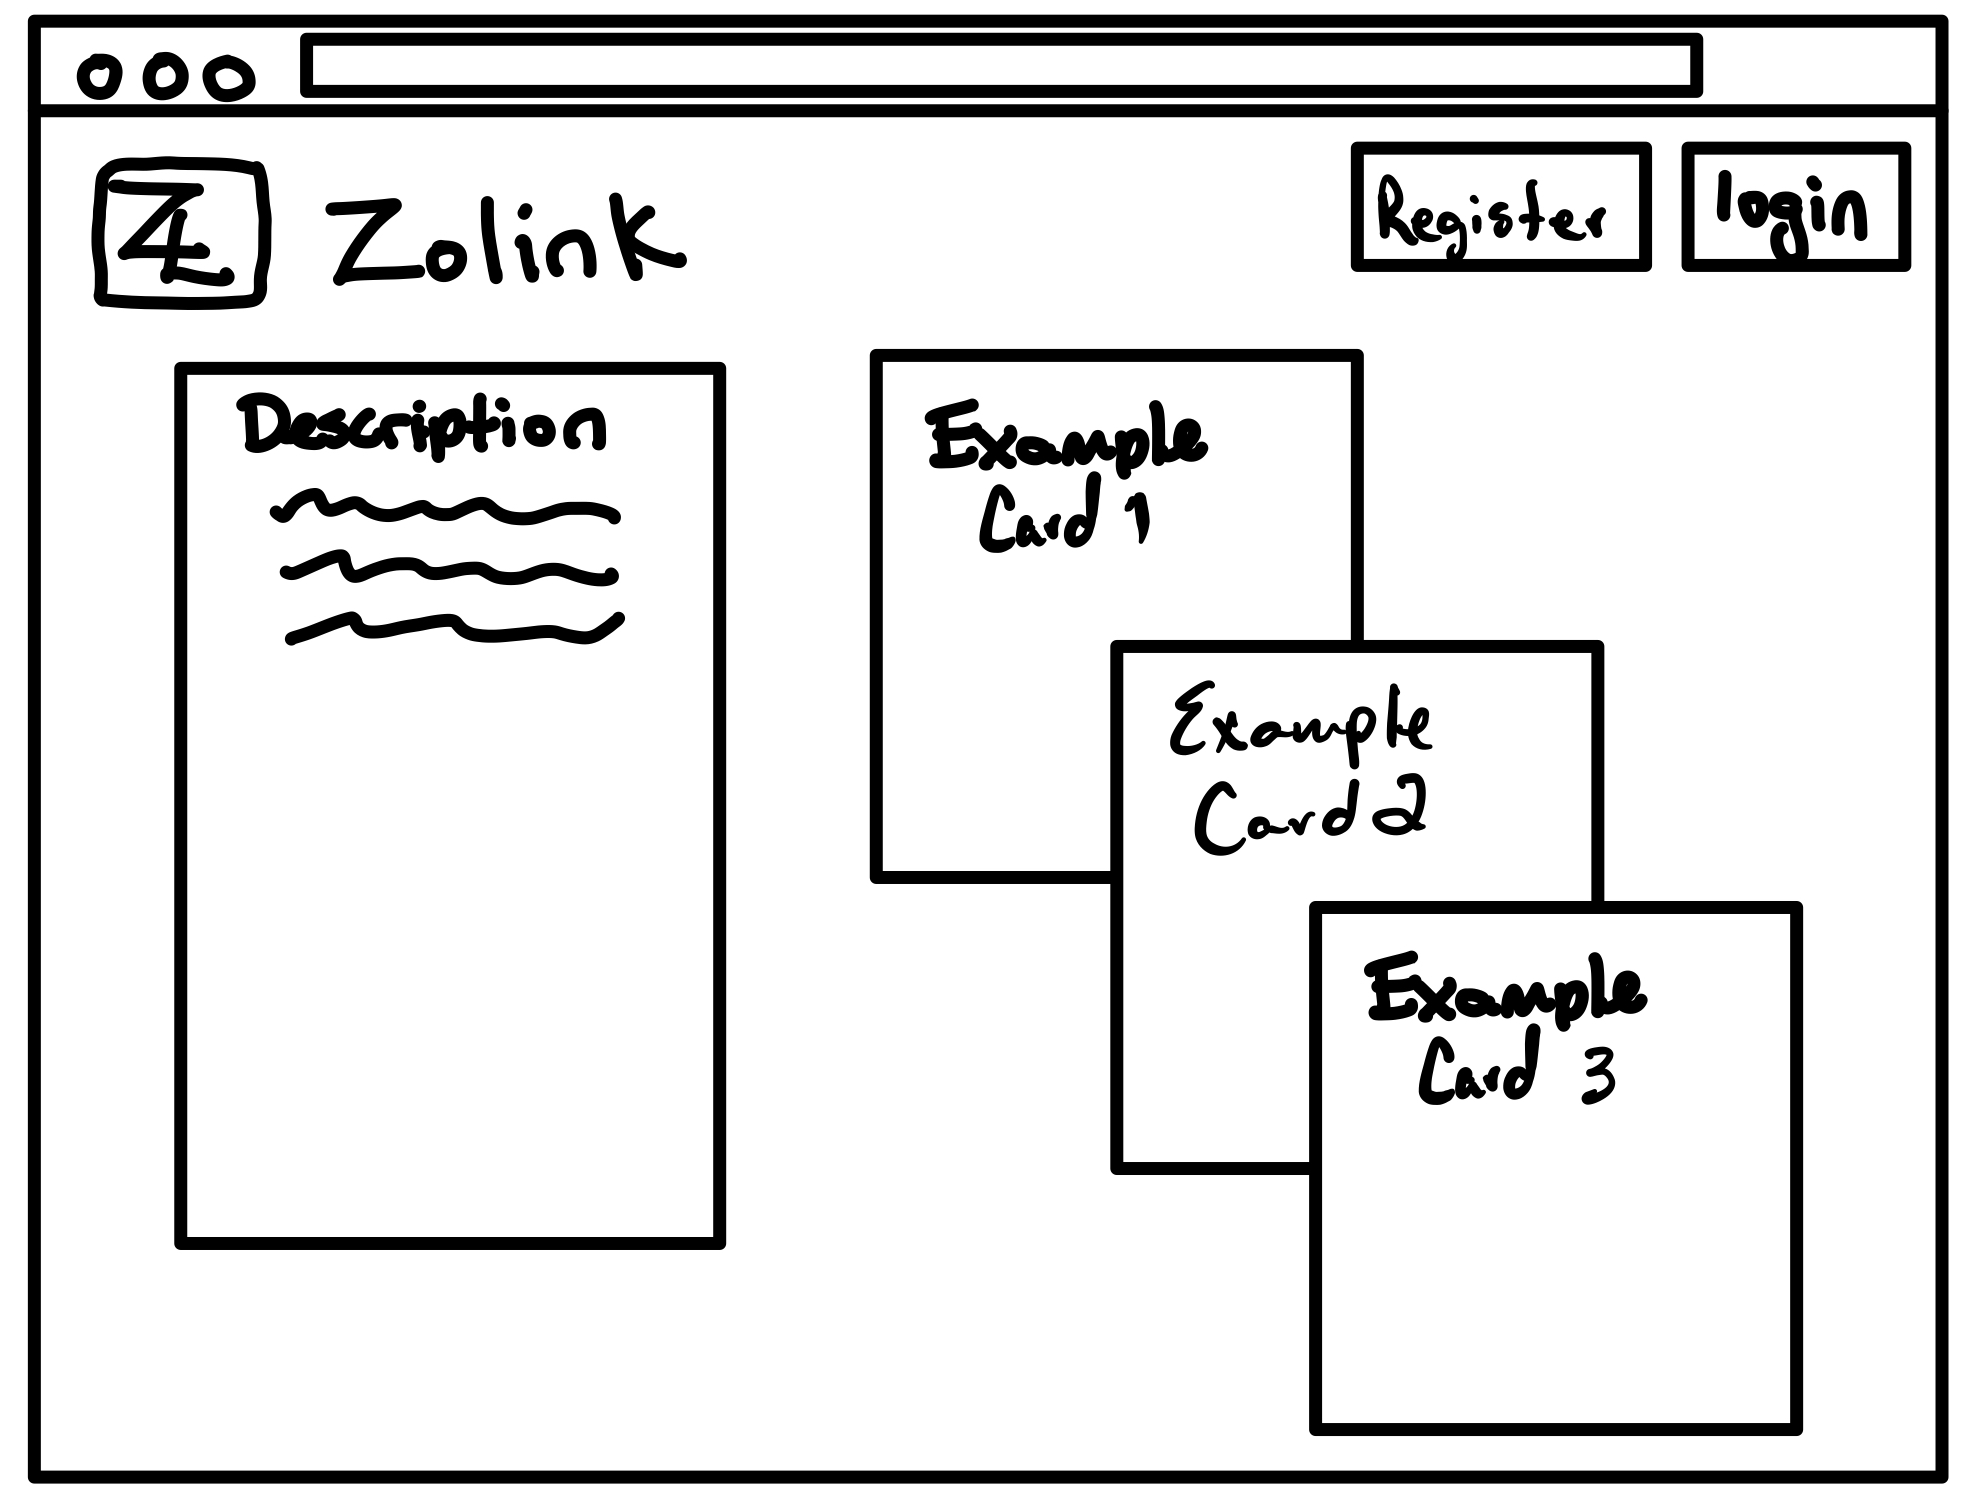
\includegraphics[width=0.98\paperwidth]{storyboard_images/welcome_page.jpeg}}
    {\it This page will provide an explanation of Zolink's purpose and show a few example cards.}
    
    \clearpage
    {\bf \Large Account Creation Page}
    \makebox[\textwidth]{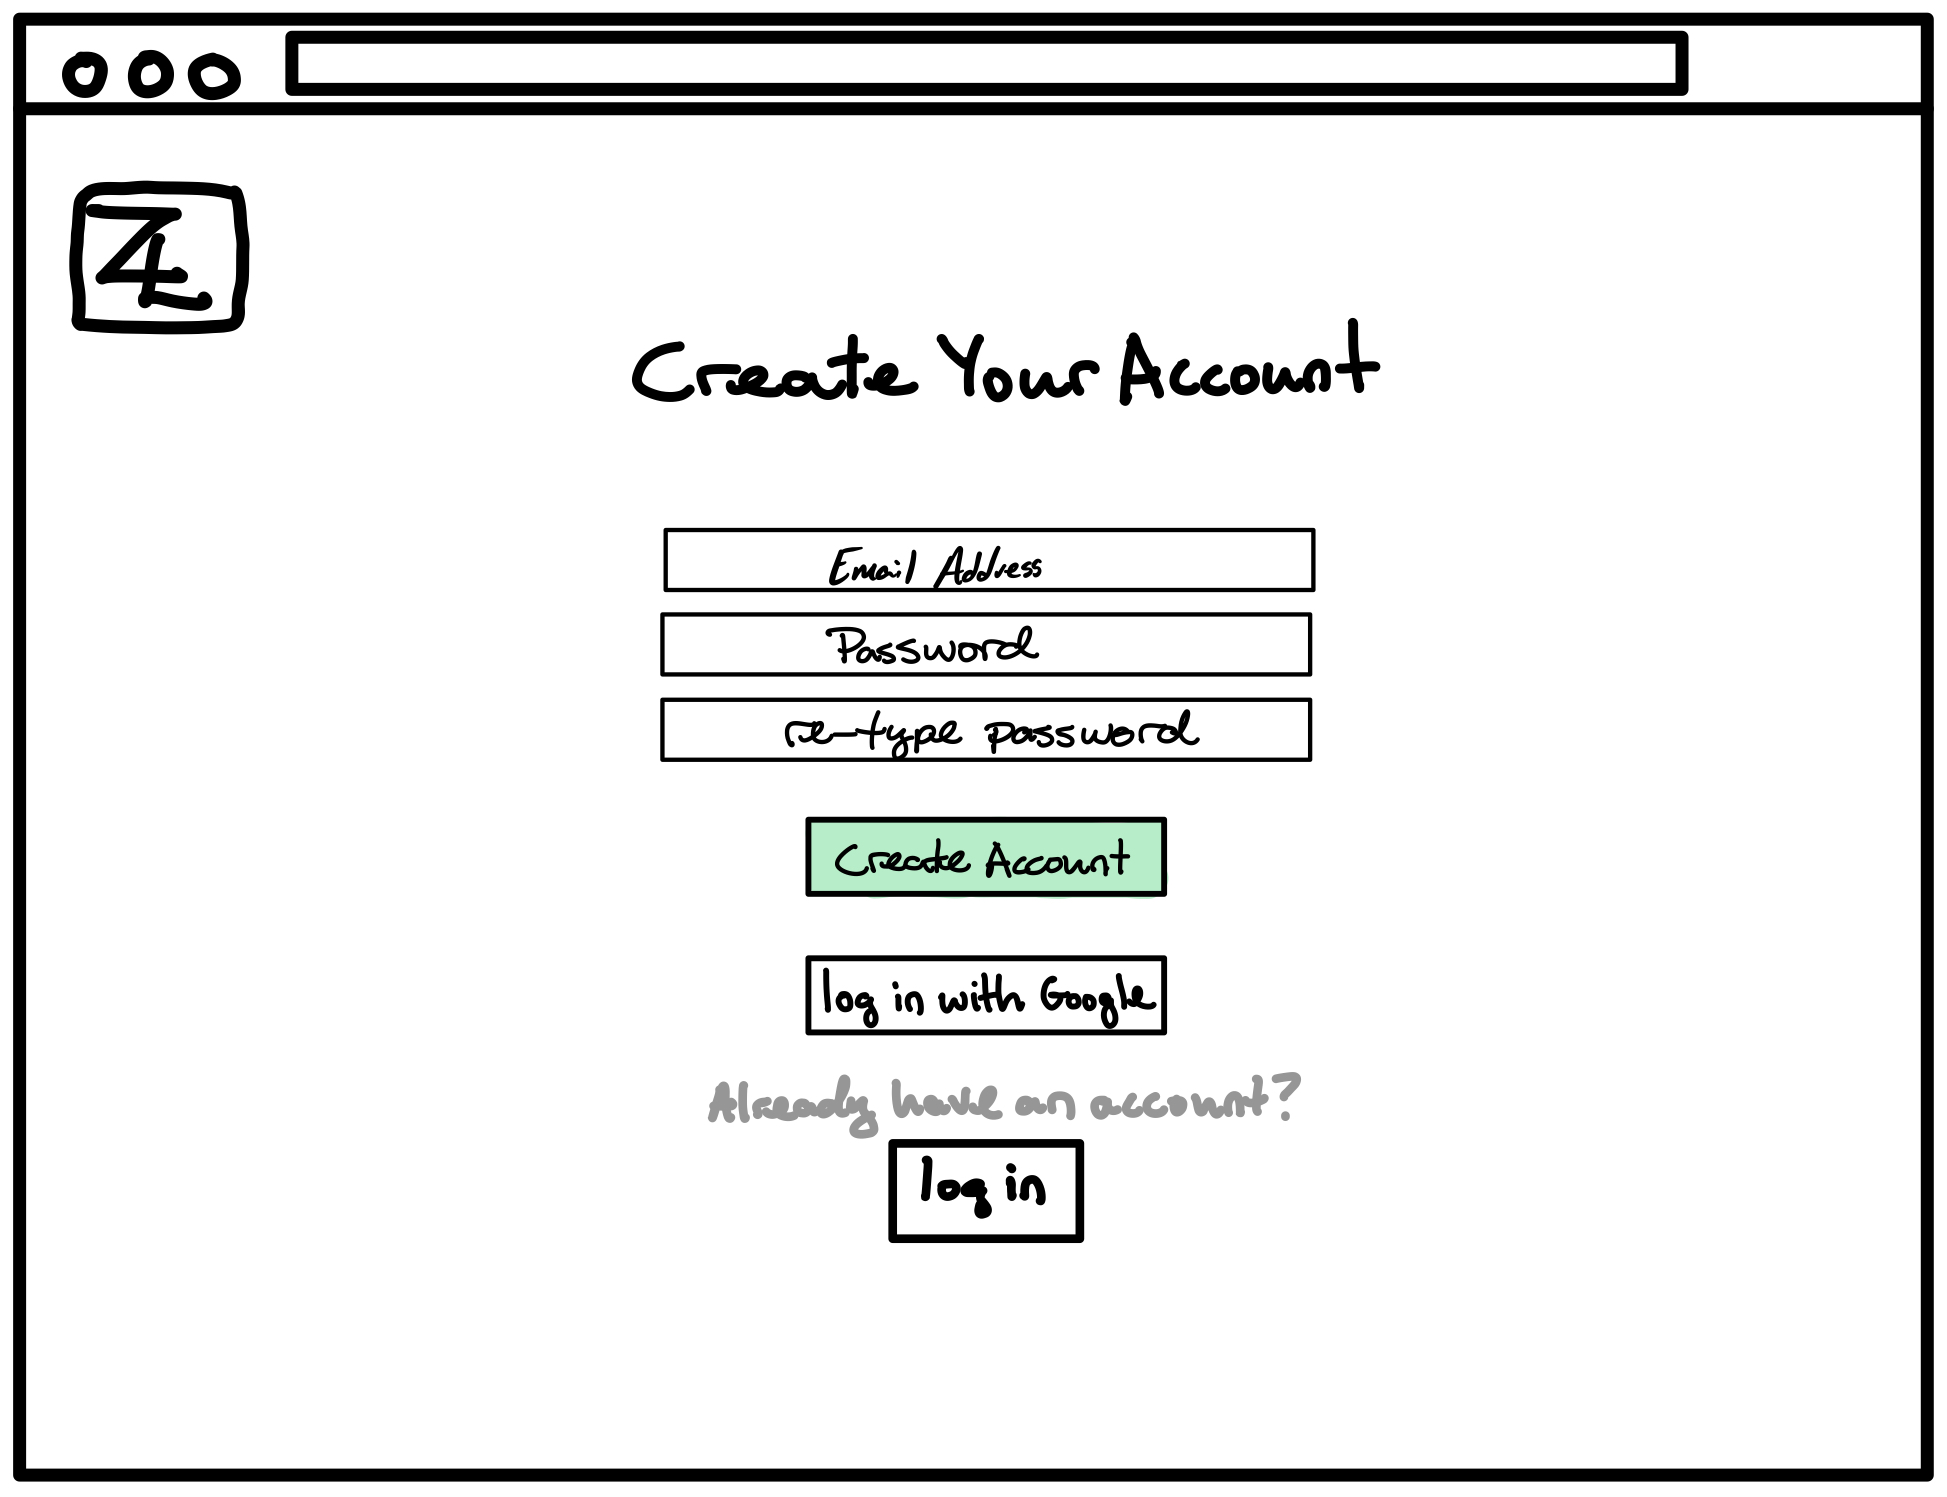
\includegraphics[width=0.98\paperwidth]{storyboard_images/account_creation.jpeg}}
    {\it NOTE: It is to be determined whether the Google login API will be included.}
    
    \clearpage
    {\bf \Large Card List Page (New Account)}
    \makebox[\textwidth]{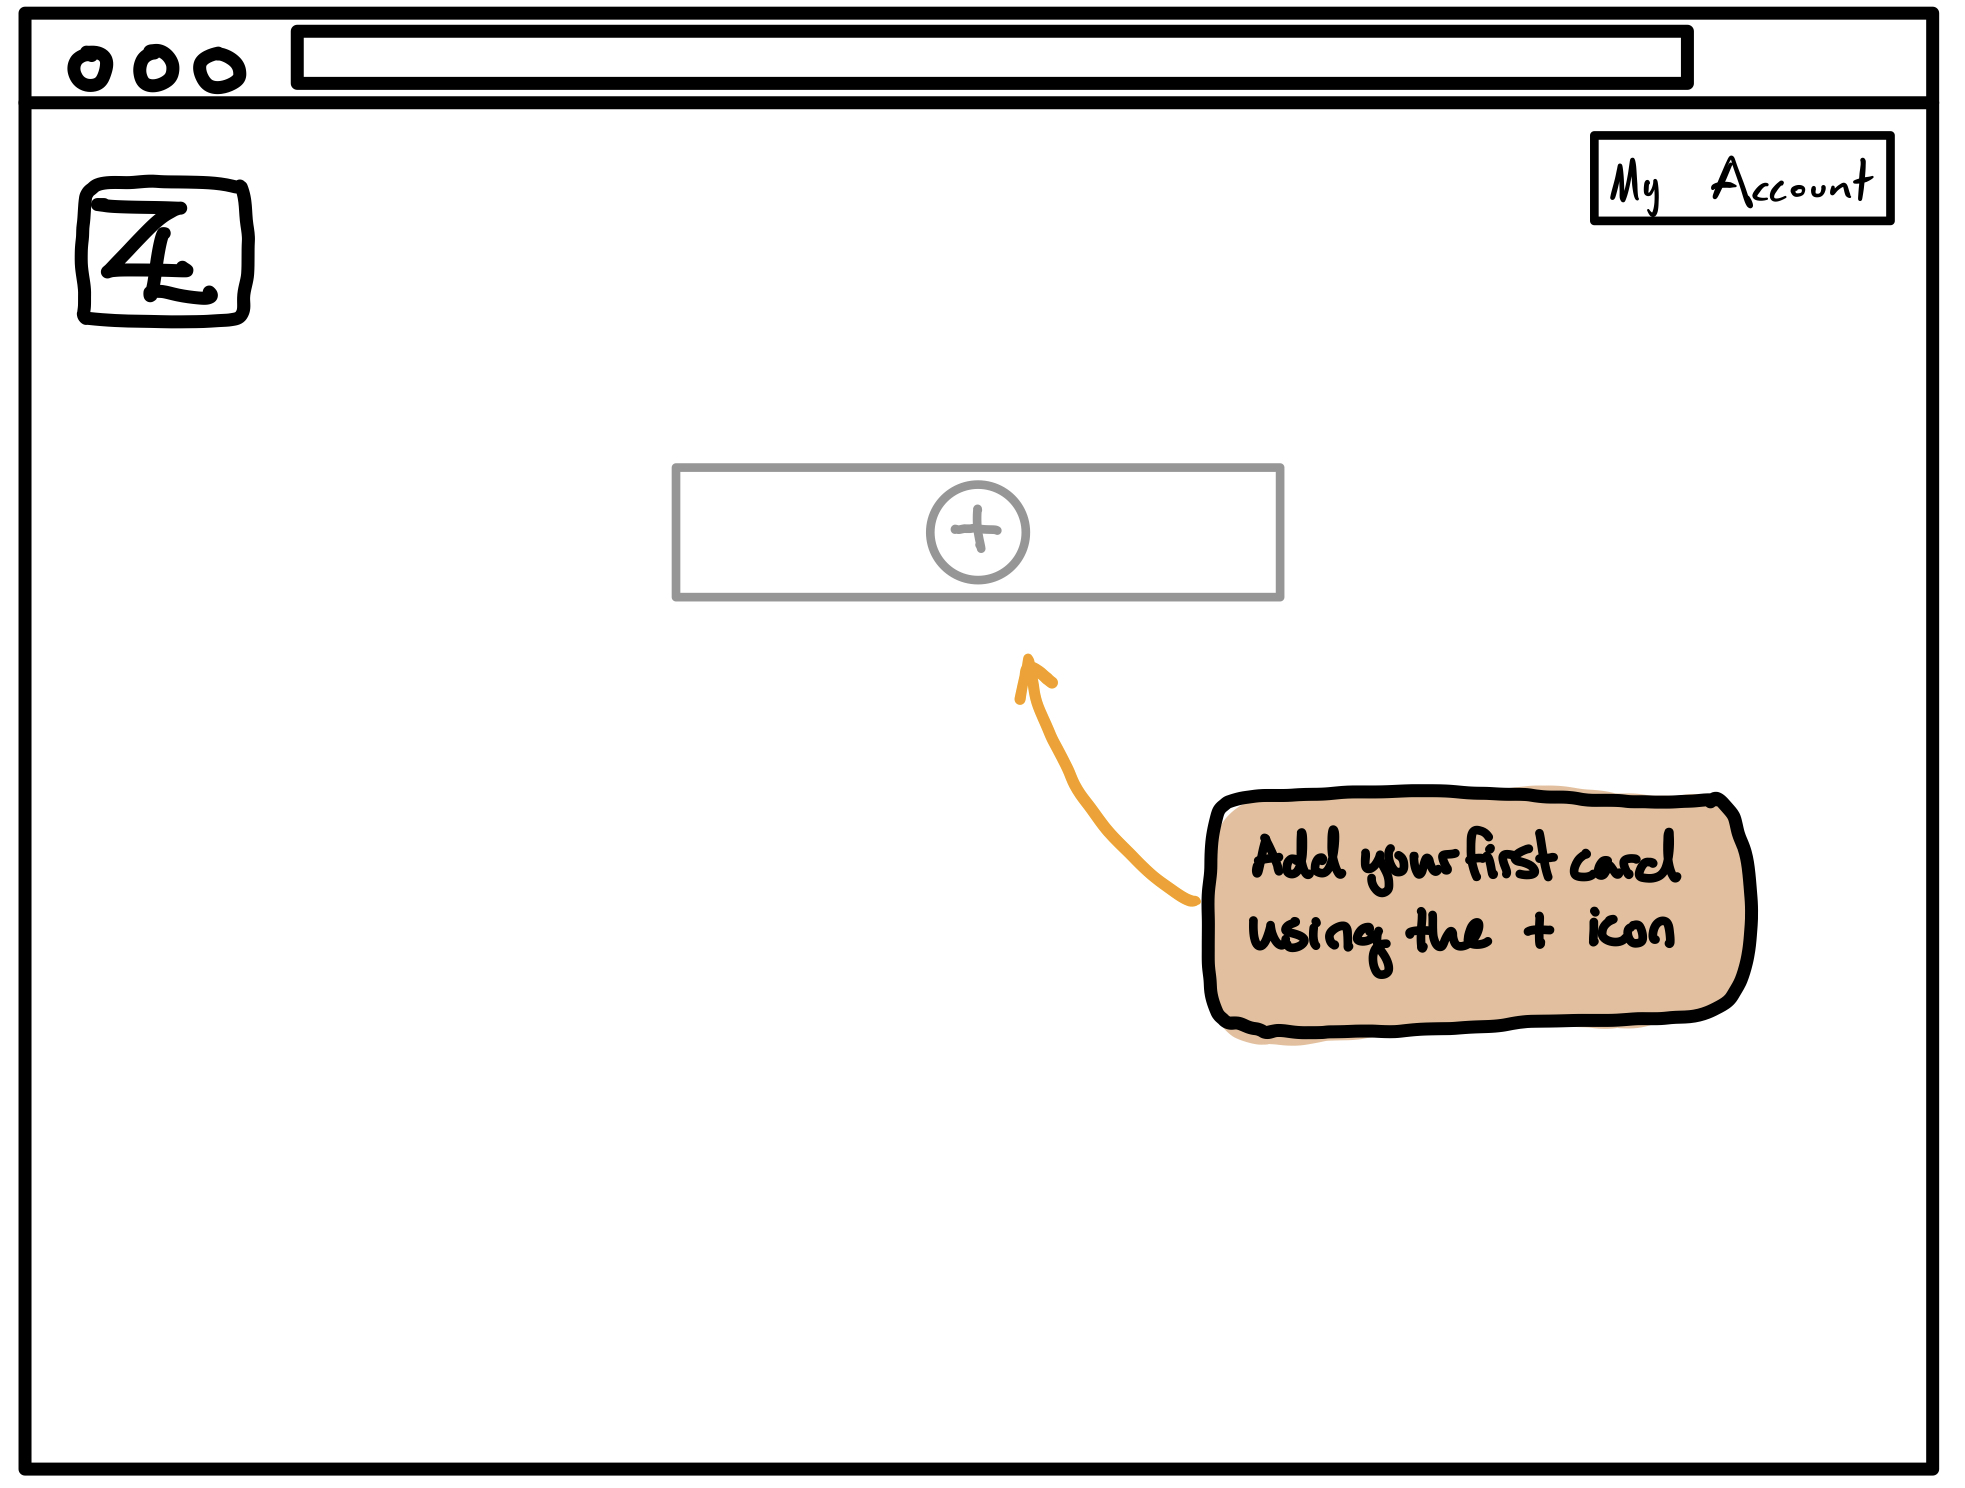
\includegraphics[width=0.98\paperwidth]{storyboard_images/card_list_page_newAcct.jpeg}}
    {\it After successfully creating an account or logging in, the user will be navigated to the Card List Page. A new account will have no cards, so only the "Add Card" button will appear on the Card List Page.}
    
    \clearpage
    {\bf \Large Create/Edit Card Page}
    \makebox[\textwidth]{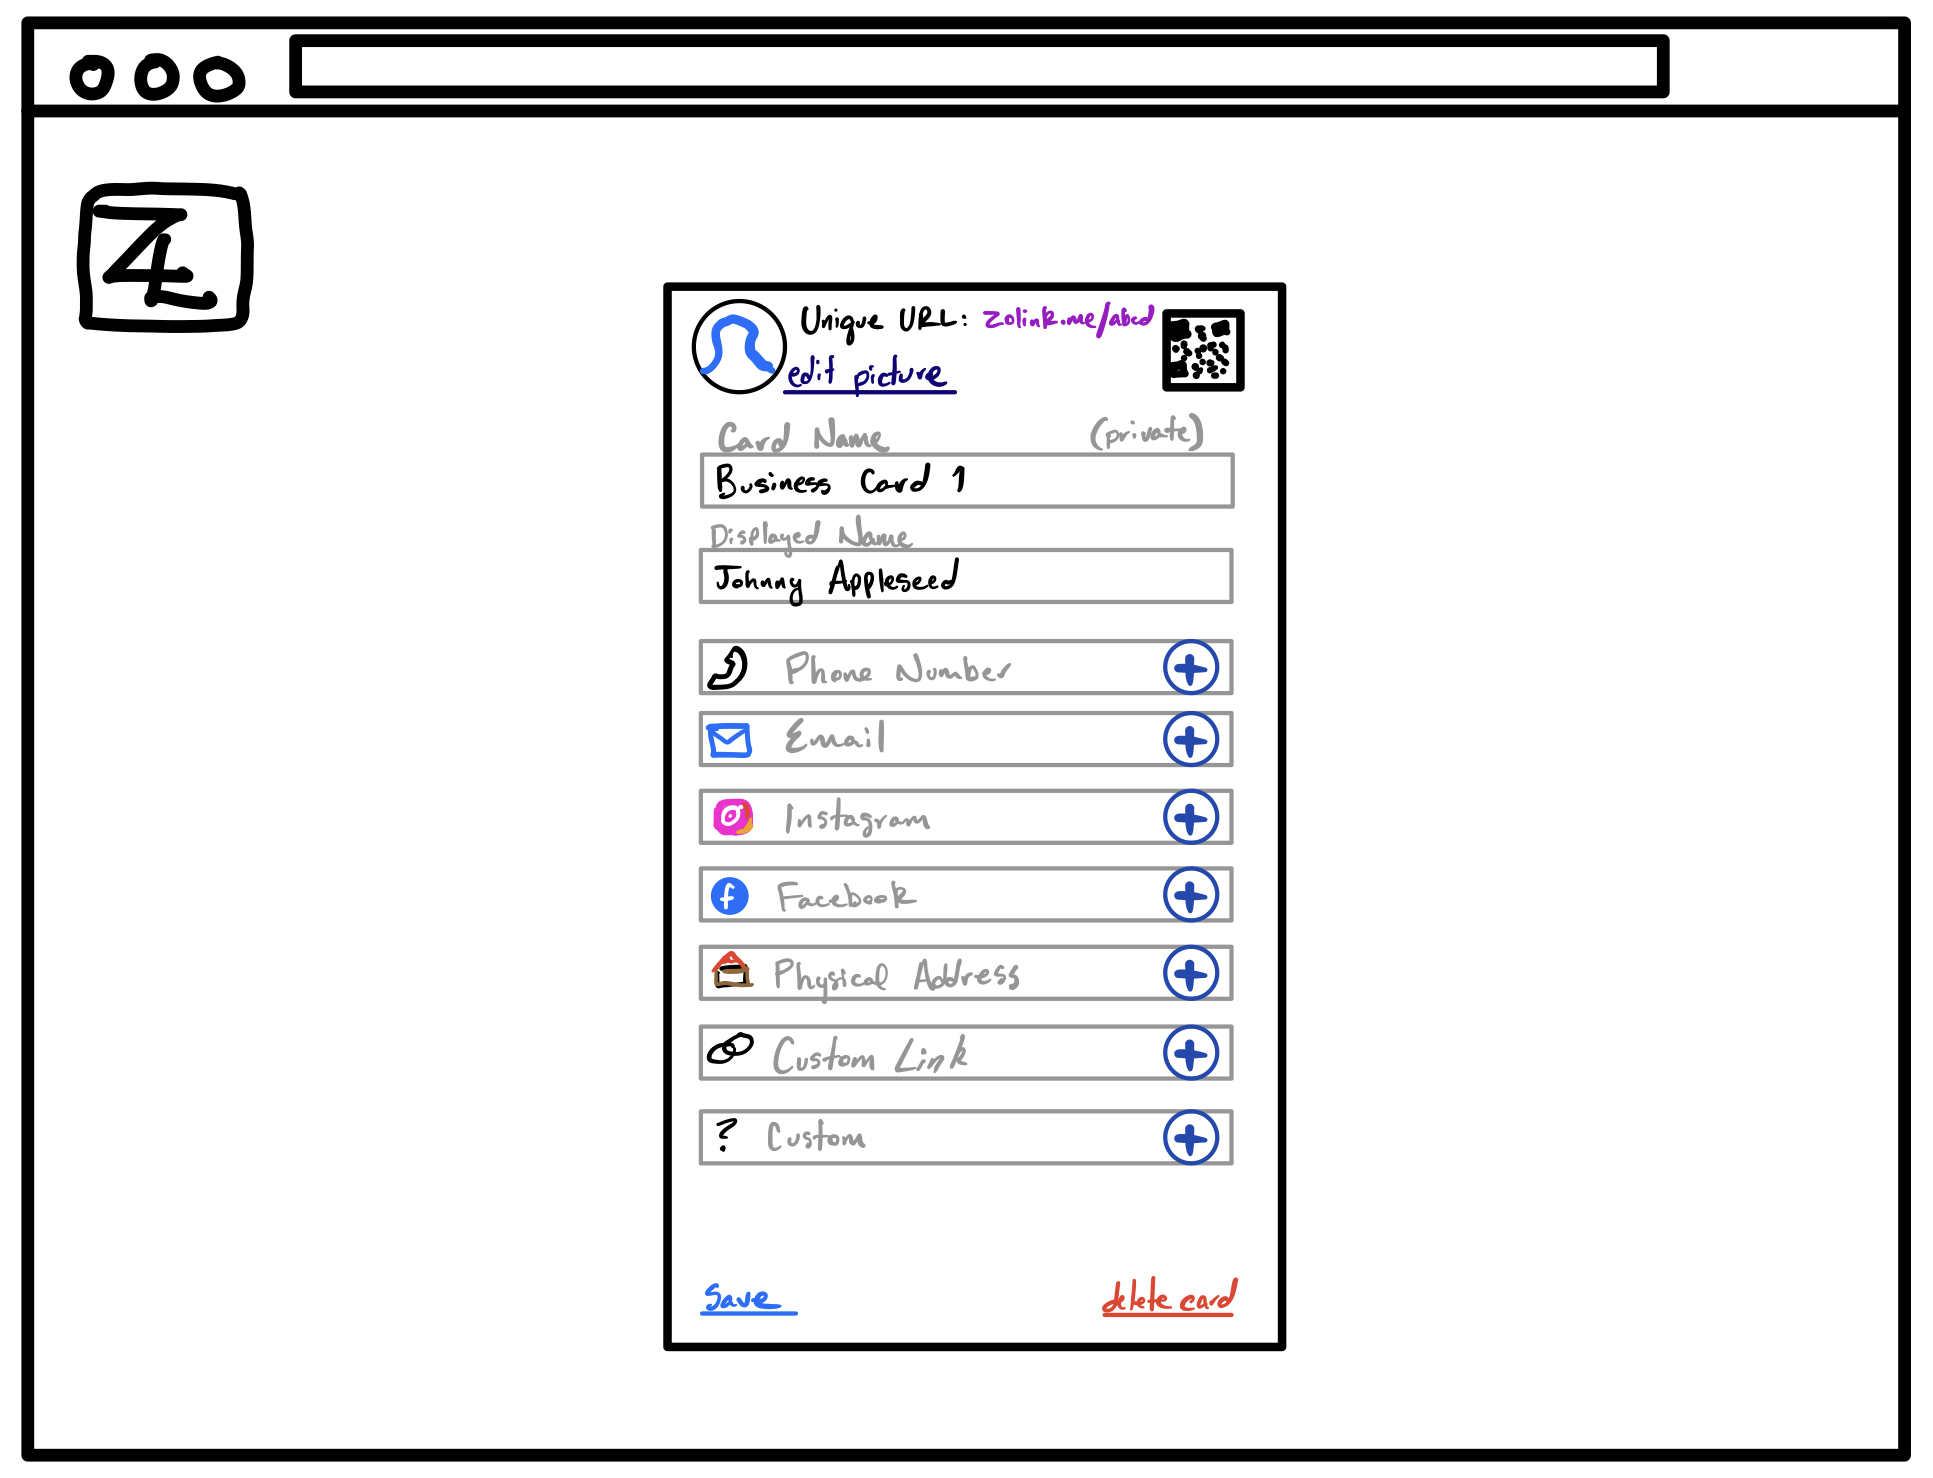
\includegraphics[width=0.98\paperwidth]{storyboard_images/create_edit_card.jpeg}}
    {\it The user can add their information to a card using this page. Attributes may be added or removed as needed.}
    
    \clearpage
    {\bf \Large Create/Edit Card Page (2)}
    \makebox[\textwidth]{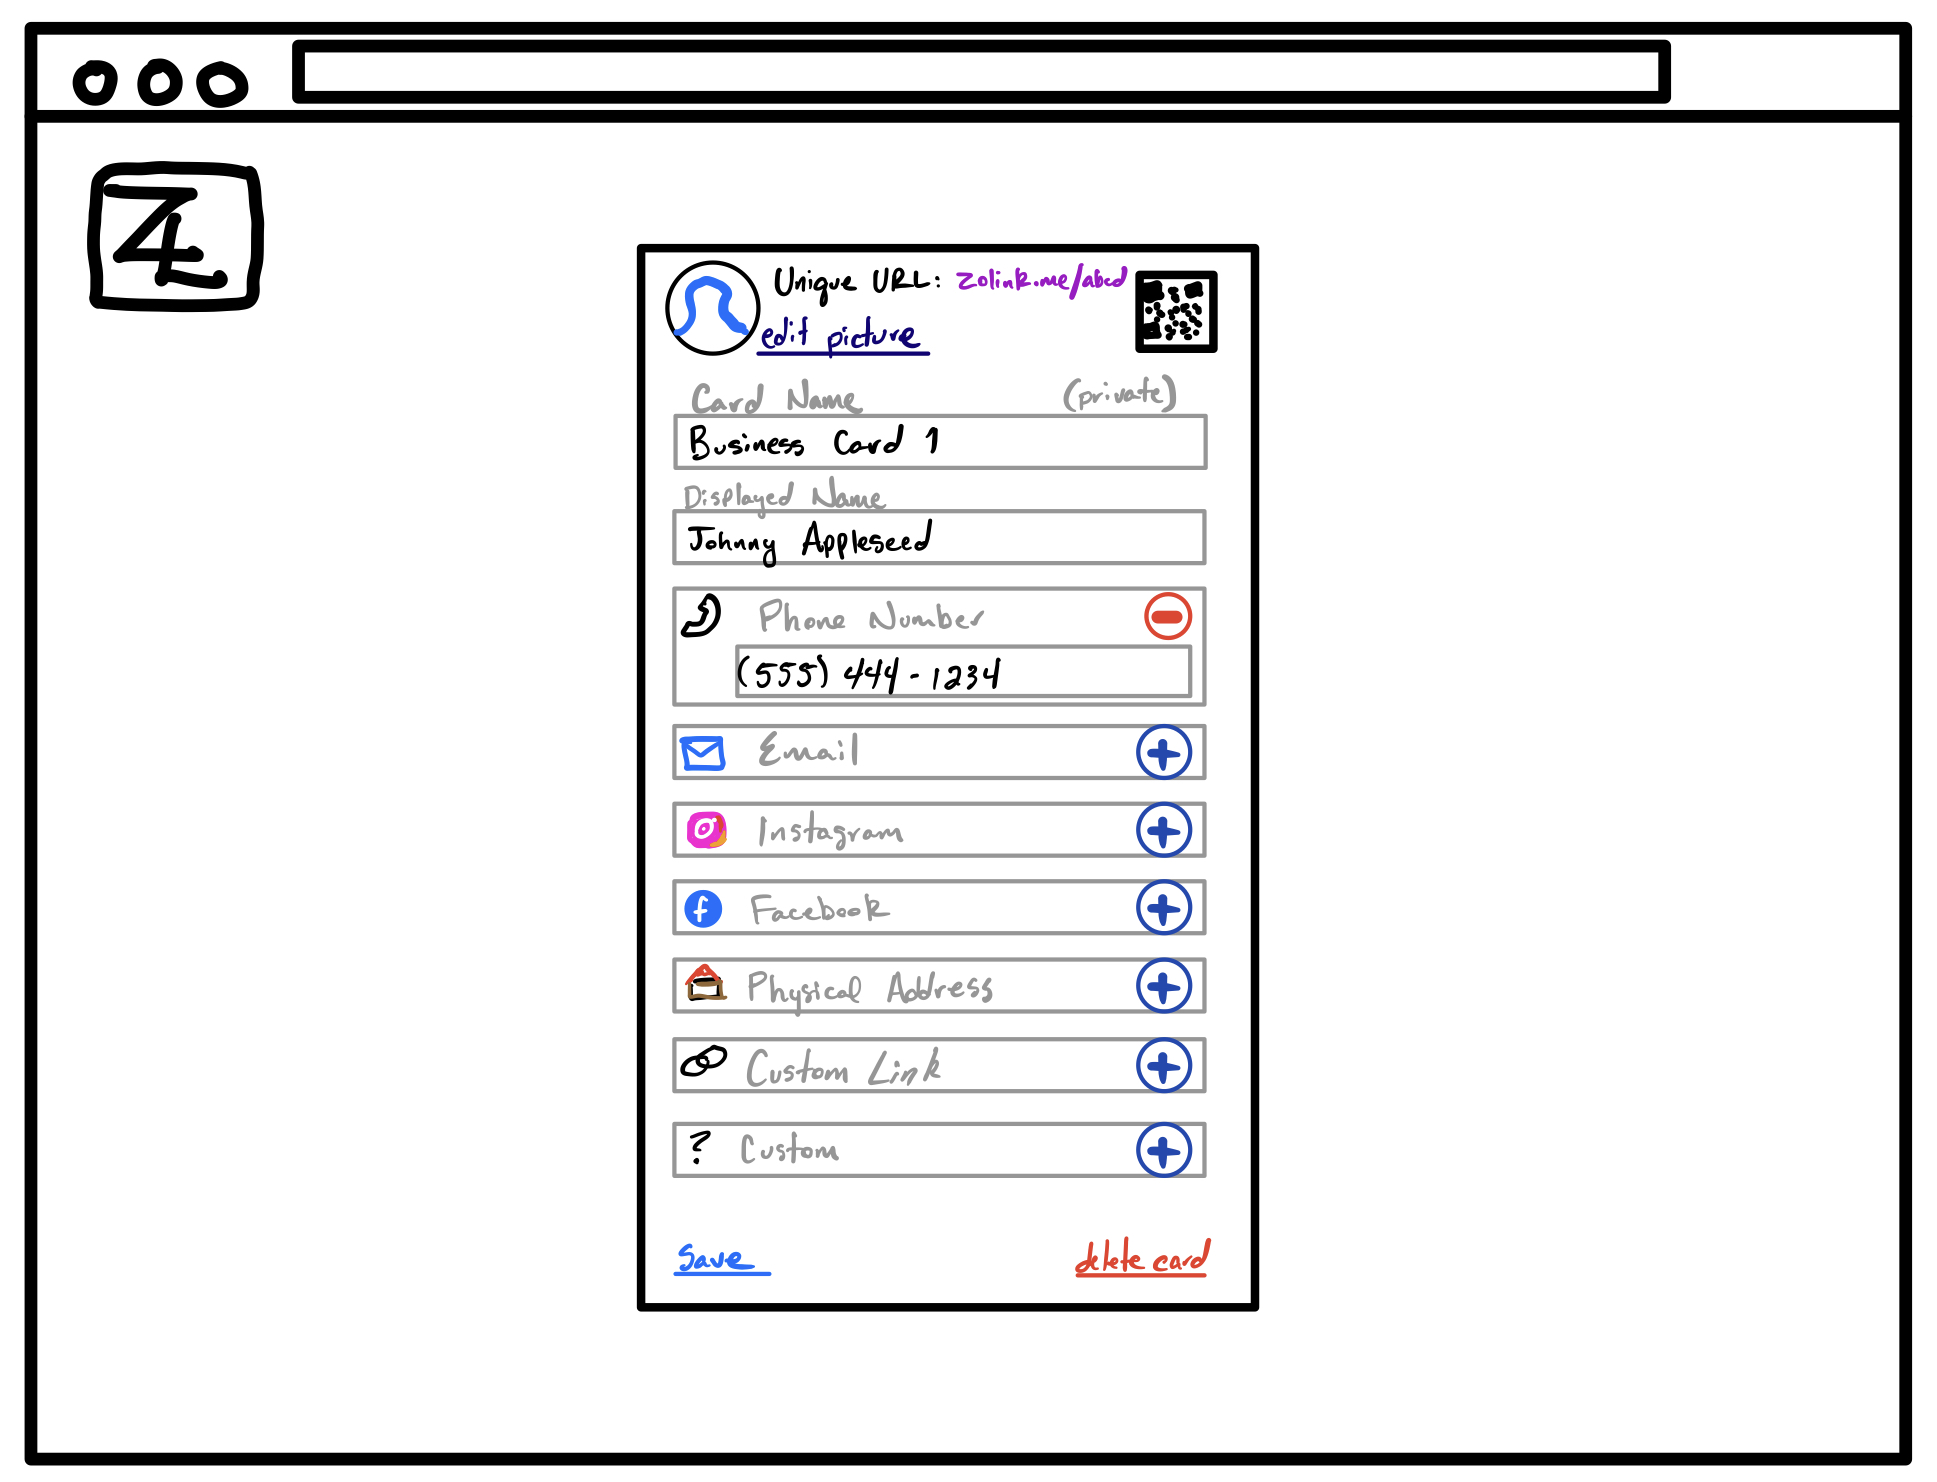
\includegraphics[width=0.98\paperwidth]{storyboard_images/create_edit_alt.jpeg}}
    {\it This sketch shows how the user will add their phone number.}
    
    \clearpage
    {\bf \Large Login Page}
    \makebox[\textwidth]{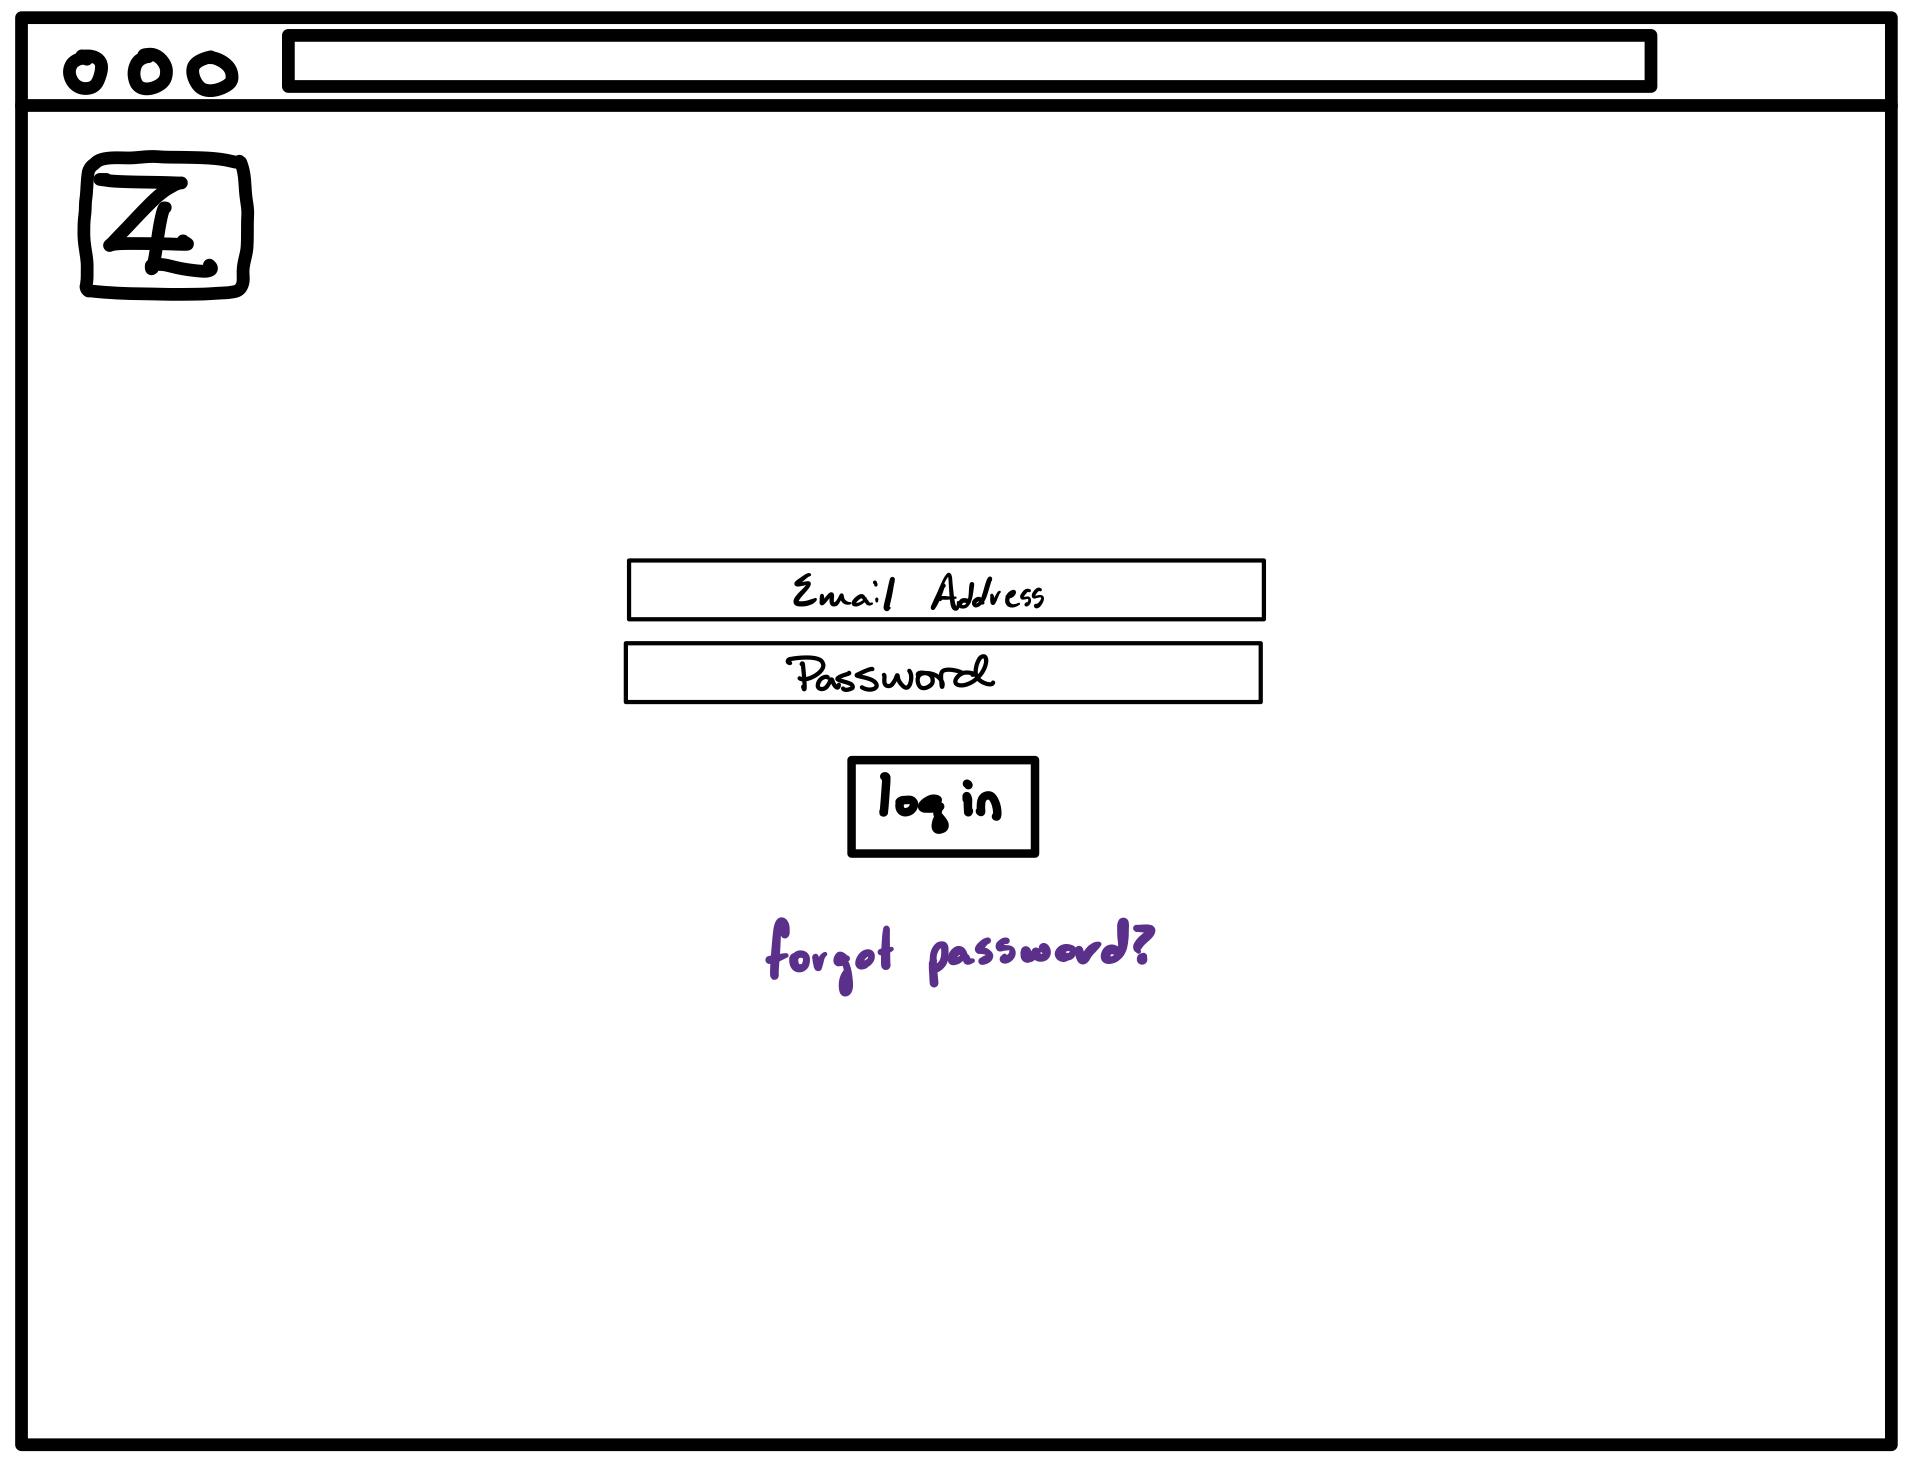
\includegraphics[width=0.98\paperwidth]{storyboard_images/login_page.jpeg}}
    
    \clearpage
    {\bf \Large Card List Page}
    \makebox[\textwidth]{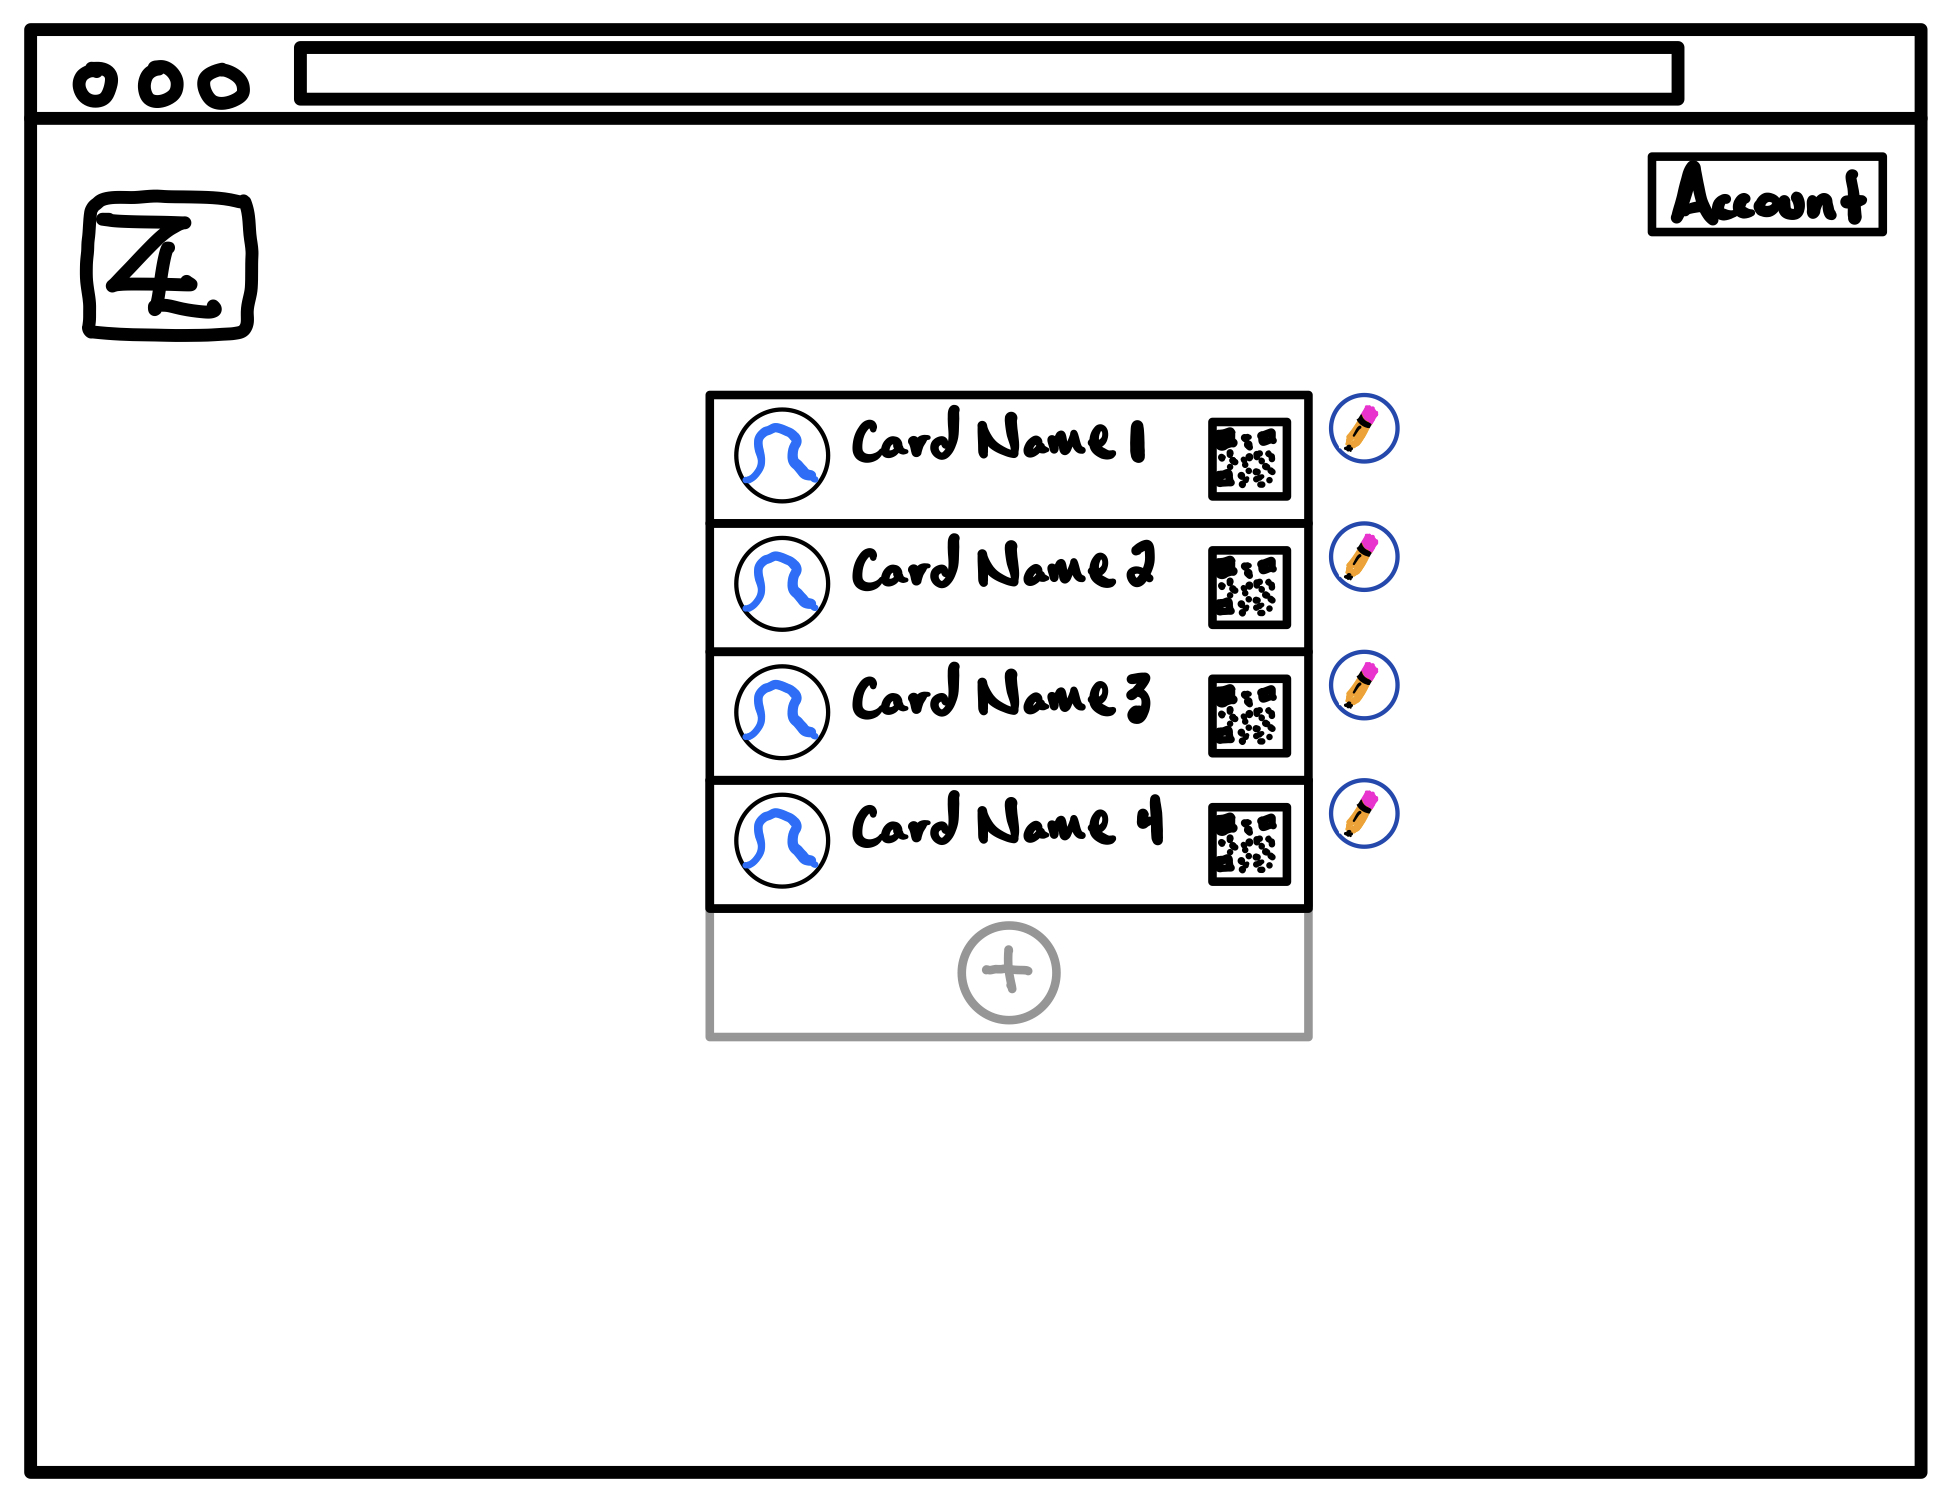
\includegraphics[width=0.98\paperwidth]{storyboard_images/card_list_page.jpeg}}
    {\it This is how the Card List Page will look after the user creates a few cards.}
    
    \clearpage
    {\bf \Large Card View Page}
    \makebox[\textwidth]{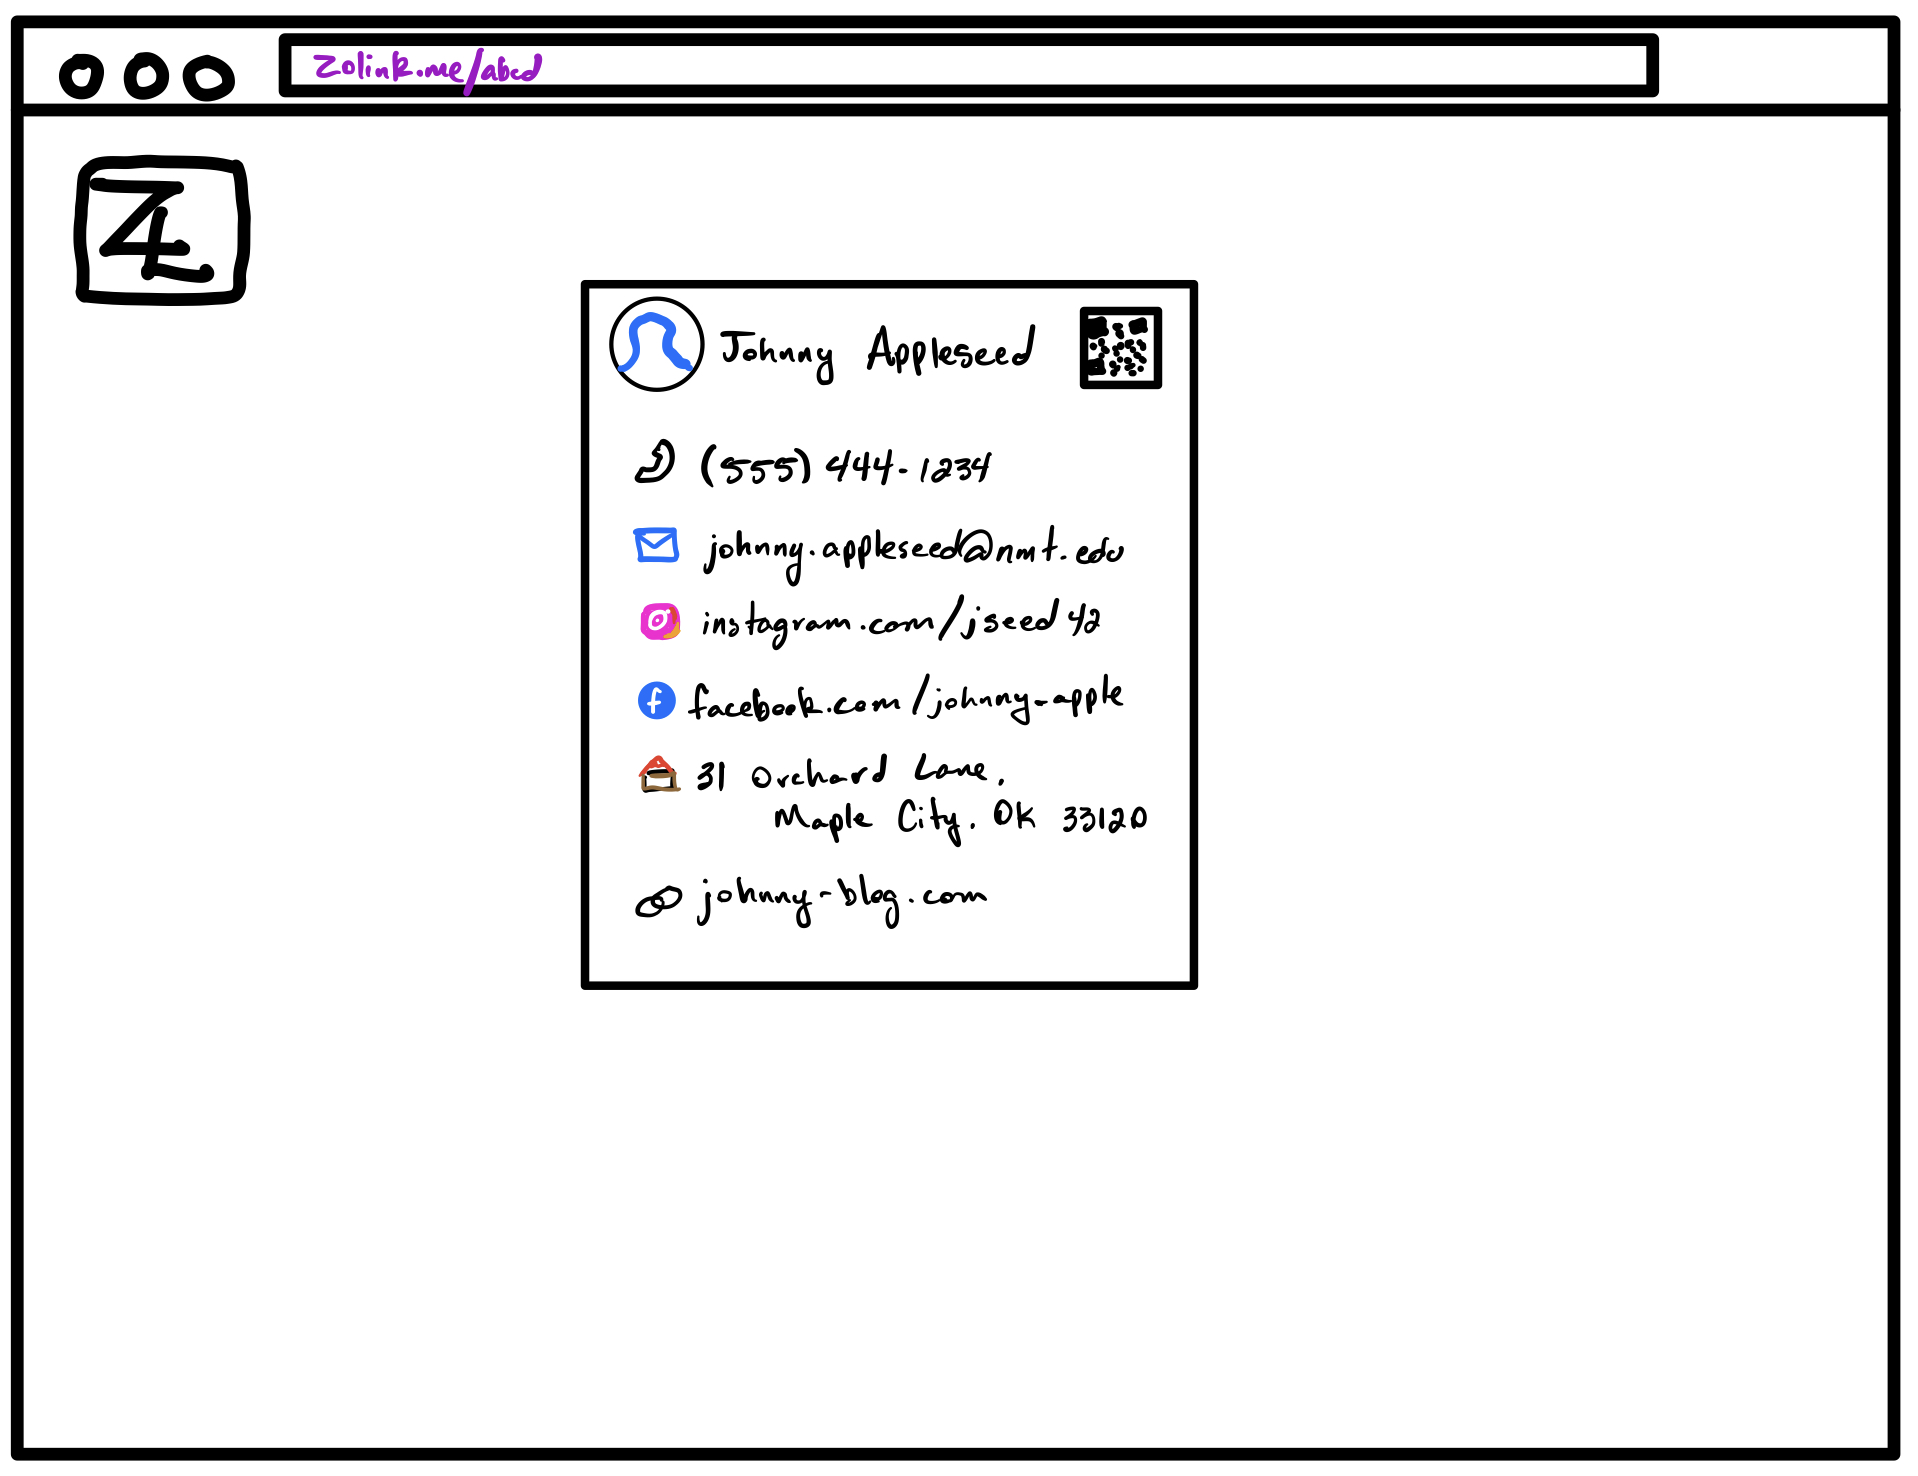
\includegraphics[width=0.98\paperwidth]{storyboard_images/card_page.jpeg}}
    {\it By clicking on one of the cards, the user may view it on this page.}
    
    \clearpage
    {\bf \Large Card QR Code View Page}
    \makebox[\textwidth]{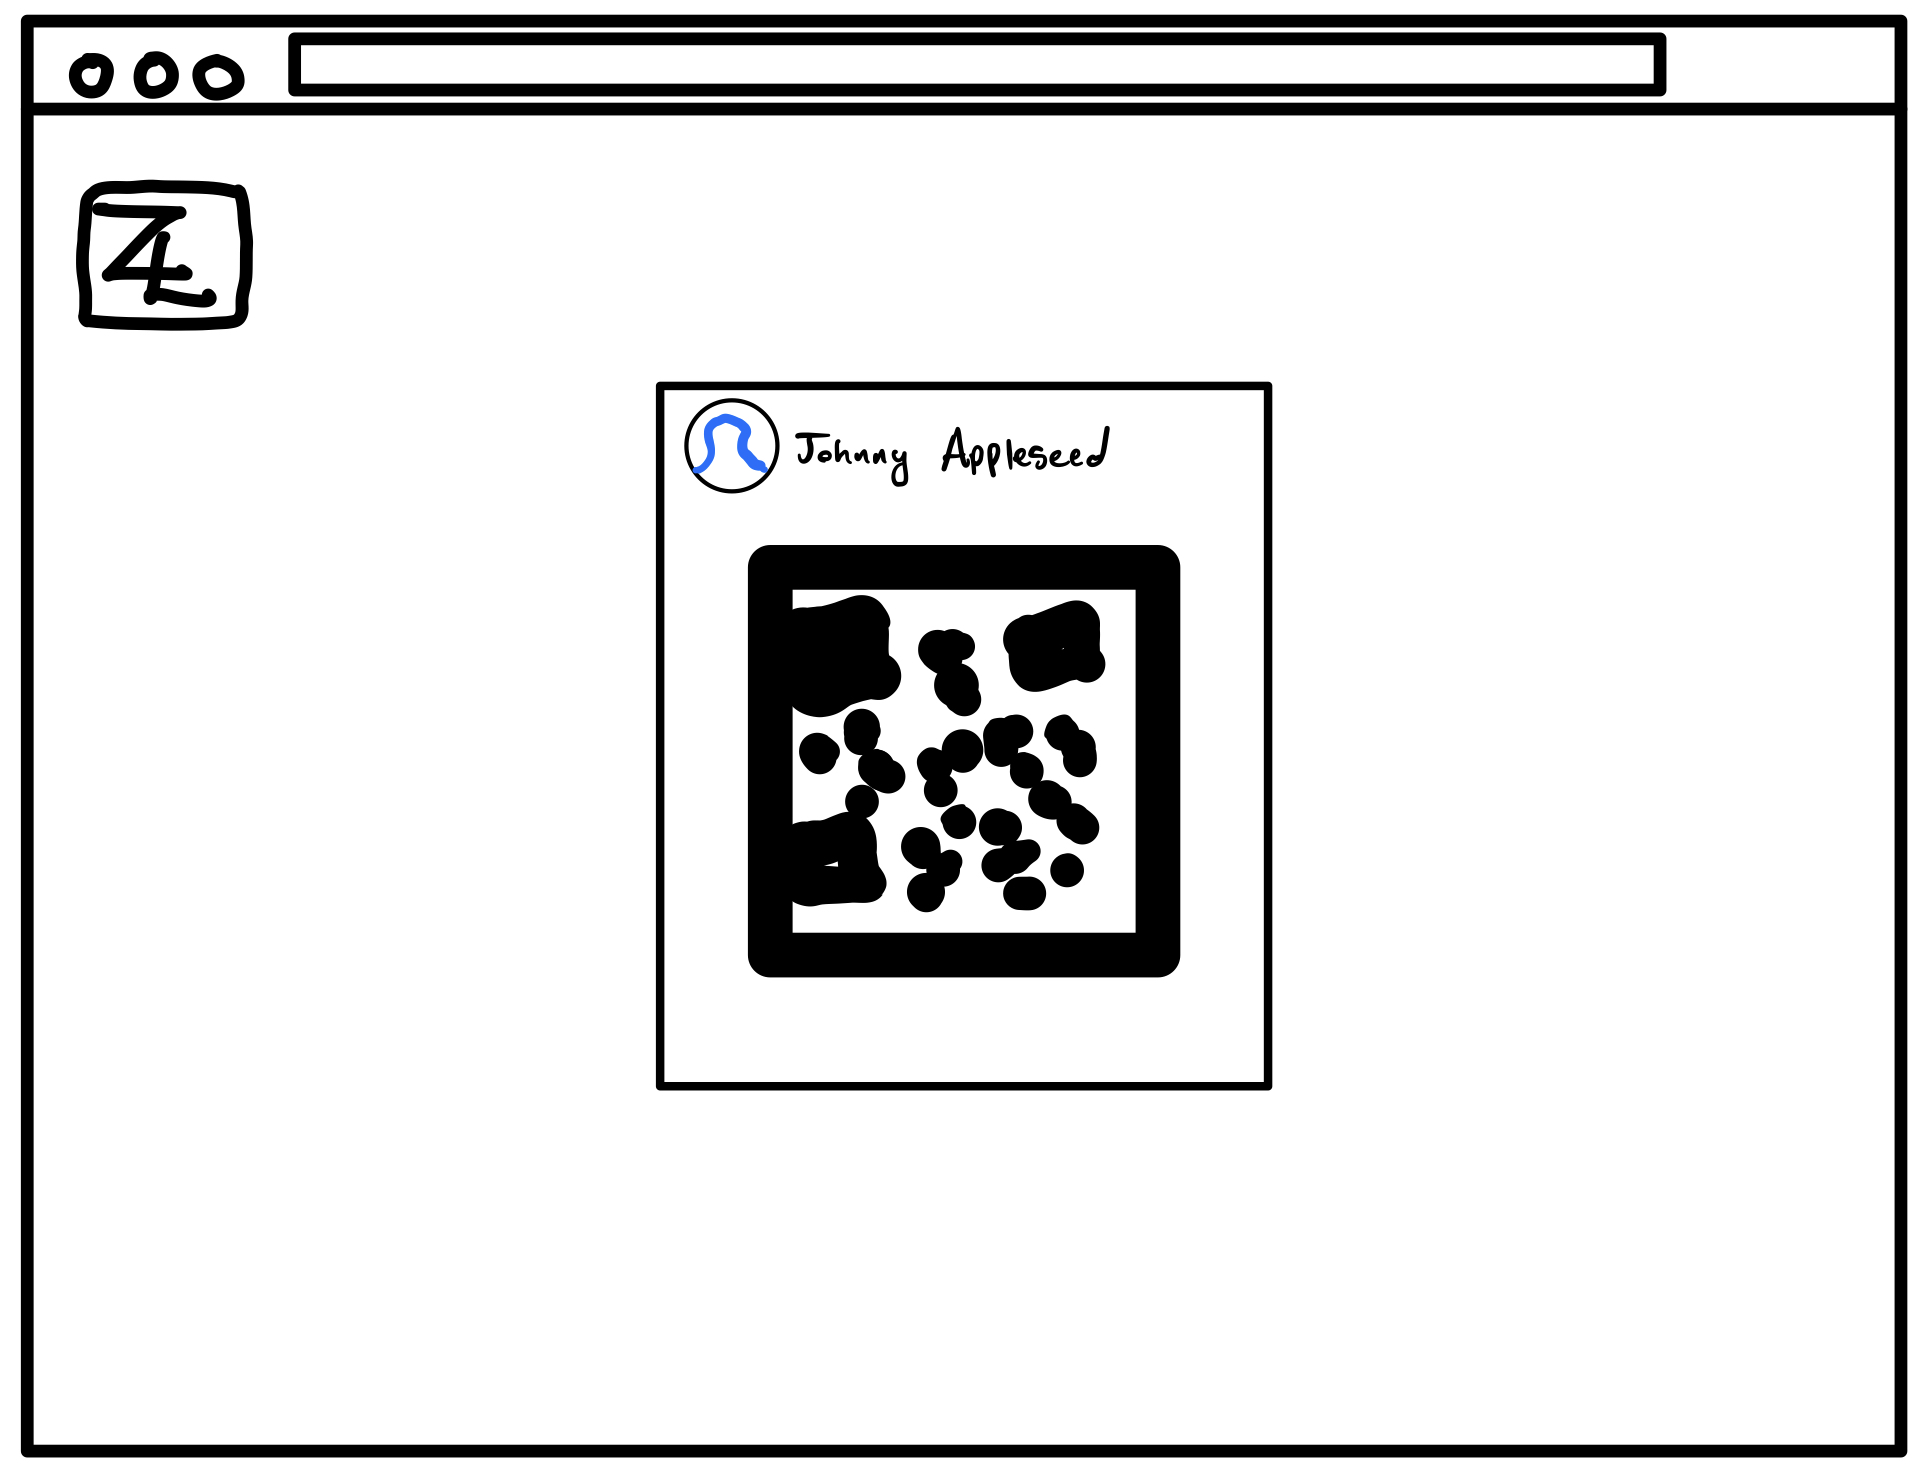
\includegraphics[width=0.98\paperwidth]{storyboard_images/qr_code_page.jpeg}}
    {\it By clicking the QR code on the Card View Page, the user may view the unique QR code for that card.}
    
    \clearpage
    {\bf \Large Account Page}
    \makebox[\textwidth]{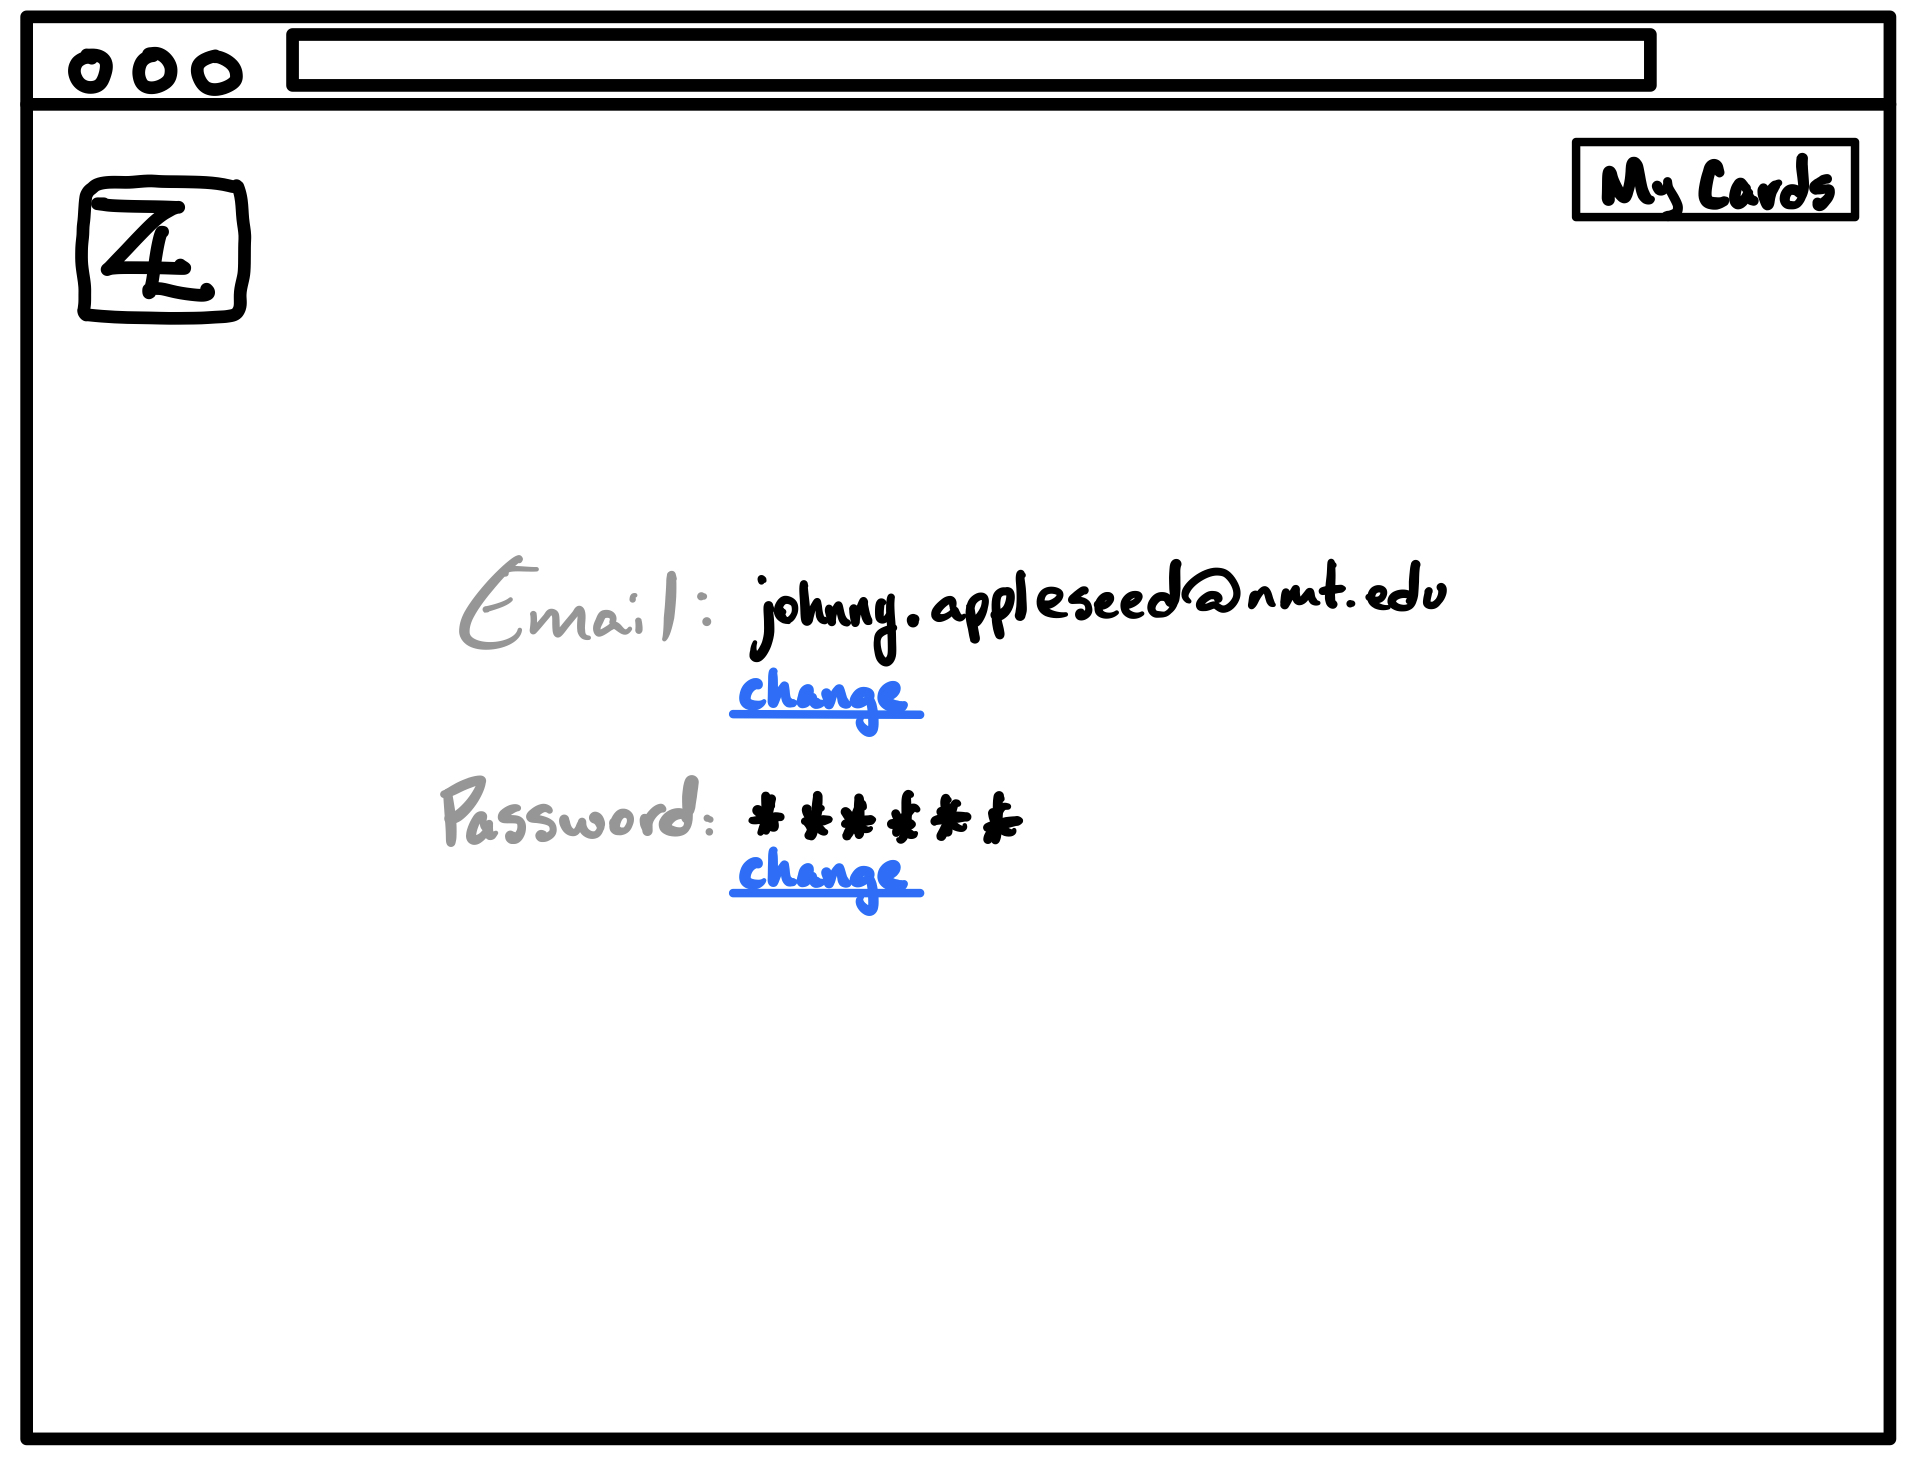
\includegraphics[width=0.98\paperwidth]{storyboard_images/account_page.jpeg}}
    {\it The user may change their email and password on this page.}
    
\end{center}

\clearpage
\section{ER Diagram}

\begin{enumerate}[4.a.]
    \item ER Diagram\\
     - Prolog explaining what is the purpose of this section.\\
     - The ER Diagram
    
    \item Table Design.\\
    In each table, you should describe following information with bullets or tables:\\
 - The fields information for each table with comments\\
 - Briefly describe why you design the table, such as why you design this field as VARCHAR.\\
 - If this table has foreign key, please describe the relation between this table and other tables.\\
    
    
\end{enumerate}

%============================================================================
\end{document}
%============================================================================
